%!TEX TS-program = xelatex
\documentclass[14pt, a4paper]{article}  
\usepackage{extsizes}


\usepackage[british,russian]{babel}
\usepackage[utf8]{inputenc} 

% шрифт
\usepackage{fontspec}  
\setmainfont{Arial}

% картинки
\usepackage{graphicx} 
\usepackage{graphics} 
\graphicspath{{images/}{pictures/}} 

% параметры листа
\usepackage[paper=a4paper,top=10mm, bottom=10mm,left=35mm,right=35mm,includefoot]{geometry}

% размер между строк
\usepackage{setspace}
\setstretch{1}

% абзацы
\setlength{\parskip}{4mm}  
\setlength{\parindent}{0cm}

% подпись
\usepackage{frcursive} 

% гиперссылка
\usepackage{hyperref} 
\hypersetup{
	unicode=true,     
	colorlinks=true,       	
	urlcolor=blue,       
}

% Счетчики
\renewcommand{\thesection}{\Asbuk{section}} 
\setcounter{section}{0}

\usepackage{titlesec}  
\titleformat{\section}
	{\bfseries\Large}
	{Приложение \thesection :}{0.5 em}{}

% Колонтитулы
\usepackage{fancyhdr} 
\pagestyle{fancy}
\addtolength{\headheight}{0.7cm}
\rhead{\thepage}
\lhead{\rightmark}
\renewcommand{\sectionmark}[1]{\markright{Приложение \thesection.\ #1}}

\begin{document}
	
\begin{titlepage}
\cfoot{}

	\begin{center}
	
\includegraphics[height=6cm]{Hogwarts.png}
	\end{center}

{\fontsize{12pt}{1cm}\selectfont 
	Мистеру Поттеру}

\vspace{2.5cm}

Дорогой мистер Поттер,\par
Мы рады проинформировать Вас, что Вам предоставлено место в Школе чародейства и волшебства «Хогвартс».\par Пожалуйста, ознакомьтесь с приложенным к данному письму списком необходимых книг и предметов.\par
Занятия начинаются 1 сентября. Ждём вашу сову не позднее 31 июля. \par
Искренне ваша, \par
{ \cursive{~~Minerva Mc gonagall~~}}\par
Минерва МакГонагалл\\
заместитель директора


\vfill
\begin{center}
	
	{\bfseries ШКОЛА ЧАРОДЕЙСТВА И ВОЛШЕБСТВА <<ХОГВАРТС>>}
	Директор: Альбус Дамблдор\\
	(Кавалер ордена Мерлина I степени, основатель Ордена Феникса,  президент Международной конфедерации магов)
	
\end{center}
	{\small Более подробно: \href{http://vhogwarts.ru}{здесь}.}

\end{titlepage}

\newpage

\thispagestyle{fancy}

\section{Список необходимых книг и предметов}

\begin{enumerate}
	\renewcommand{\labelenumi}
	{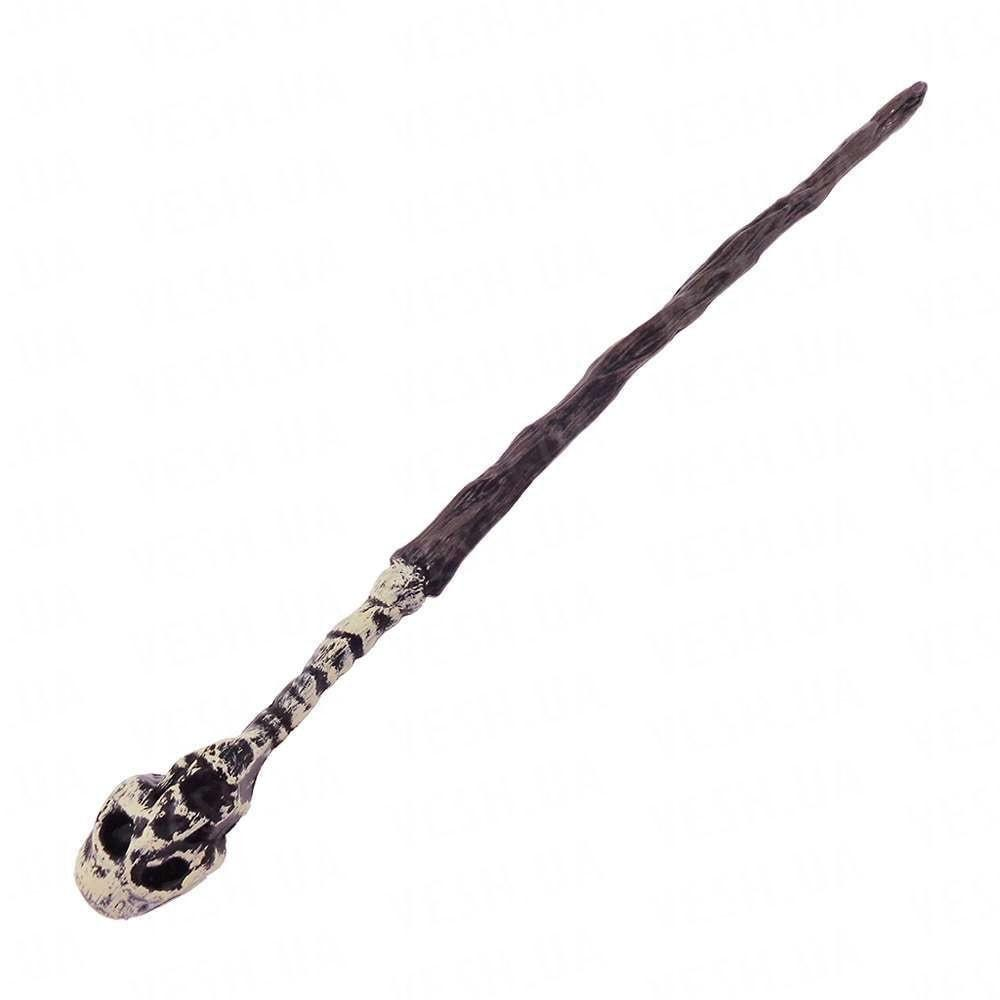
\includegraphics[scale=0.02]{palka.jpg}}
\item Волшебная палочка
\item Мантия невидимка
\item Носко <<Эконометрика>> (Книга 1 и 2)
\item Ключ от тайной комнаты
\end{enumerate}

\vfill 
\begin{center}
	{\small \bfseries Школа чародейства и волшебства <<Хогвардс>>}
\end{center}


\newpage
\section{Список изучаемых предметов}
\begin{enumerate}
	\renewcommand{\labelenumi}
	{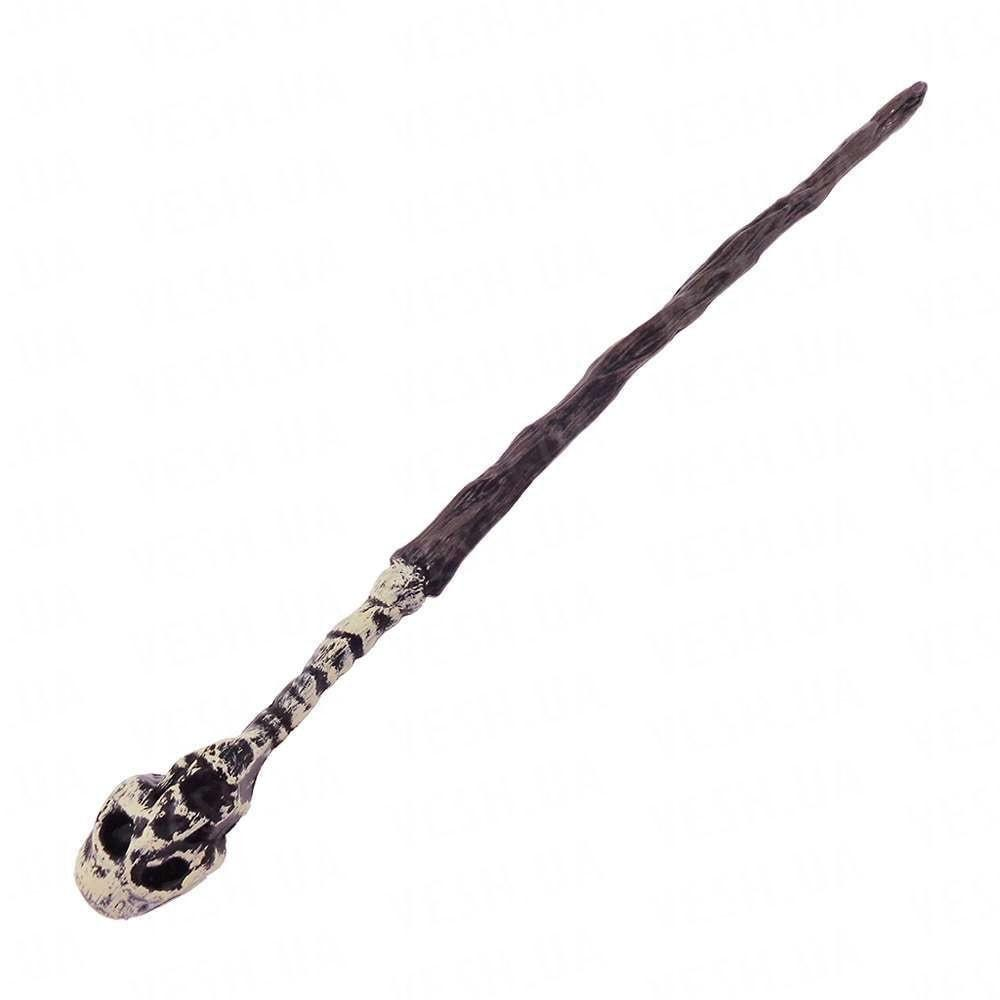
\includegraphics[scale=0.02]{palka.jpg}}
	\item Культура речи с фантастическими тварями
	\item Машиноведение
	\item Полеты на метлах
\end{enumerate}

\vfill 
\begin{center}
{\small \bfseries Школа чародейства и волшебства <<Хогвардс>>}
\end{center}

\end{document}